\documentclass{sig-alternate-05-2015}

 \usepackage{graphicx}

% \usepackage{url}
% \urldef{\mailsa}\path|{brendan.annable, mitchell.metcalfe, monica.olejniczak}@uon.edu.au|

% % Header and footer
% \usepackage{fancyhdr}
% \fancyhf{}
% \renewcommand{\headrulewidth}{0pt}
% \pagestyle{fancy}
% \cfoot{\thepage}

% Figures
\usepackage{subfigure}

% Tables
\usepackage[table]{xcolor}
\usepackage{booktabs}
\usepackage{tabularx}

\newcommand{\scarequotes}[1]{`#1'}
\newcommand{\newterm}[1]{{\textit{#1}}}

% References
%\usepackage{natbib}
% \makeatletter
% 	% Change natbib numbering style from [#] to #.
% 	\renewcommand\@biblabel[1]{#1.}
% 	% Reset bibsection so references appear correctly
% 	\renewcommand\bibsection%
% 	{
% 	  \section*{\refname
% 		\@mkboth{\MakeUppercase{\refname}}{\MakeUppercase{\refname}}}
% 	}
% \makeatother

% TODO: Fix citation commands.
\newcommand{\citep}[1]{\cite{#1}}
\newcommand{\citet}[1]{\cite{#1}}

% To-do notes:
\usepackage[disable]{todonotes}
\presetkeys{todonotes}{inline}{}

% Other
\usepackage{hyperref}
\usepackage{float}

\usepackage{pgfplots}
\pgfplotsset{width=\textwidth,compat=1.9}

\begin{document}

	% TODO: Fix metadata.

	% Copyright
	\setcopyright{acmcopyright}
	%\setcopyright{acmlicensed}
	%\setcopyright{rightsretained}
	%\setcopyright{usgov}
	%\setcopyright{usgovmixed}
	%\setcopyright{cagov}
	%\setcopyright{cagovmixed}


	% DOI
	\doi{10.475/123_4}

	% ISBN
	\isbn{123-4567-24-567/08/06}

	%Conference
	\conferenceinfo{PLDI '13}{June 16--19, 2013, Seattle, WA, USA}

	\acmPrice{\$15.00}

	%
	% --- Author Metadata here ---
	\conferenceinfo{WOODSTOCK}{'97 El Paso, Texas USA}
	%\CopyrightYear{2007} % Allows default copyright year (20XX) to be over-ridden - IF NEED BE.
	%\crdata{0-12345-67-8/90/01}  % Allows default copyright data (0-89791-88-6/97/05) to be over-ridden - IF NEED BE.
	% --- End of Author Metadata ---

	% \title{Sphere Detection using Boosted Classifiers}
	% \titlerunning{Sphere Detection using Boosted Classifiers}
	% \author{Brendan Annable, Mitchell Metcalfe, and Monica Olejniczak}
	% \authorrunning{B. Annable, M. Metcalfe, and M. Olejniczak}
	%
	% \institute{School of Electrical Engineering and Computer Science \\
	% 			Faculty of Engineering and Built Environment \\
	% 			The University of Newcastle, Callaghan, NSW, 2308, Australia. \\
	% 			\mailsa \\}
	%
	% \toctitle{Sphere Detection using Boosted Classifiers}
	% \tocauthor{B. Annable, M. Metcalfe, and M. Olejniczak}
	% % \maketitle
	% % \thispagestyle{plain}

	%\title{Sphere Detection using Boosted Classifiers}
	\title{A Study on Spherical Ball Detection using Boosted Classifiers}
	% \subtitle{[Extended Abstract]
	% \titlenote{A full version of this paper is available as
	% \textit{Author's Guide to Preparing ACM SIG Proceedings Using
	% \LaTeX$2_\epsilon$\ and BibTeX} at
	% \texttt{www.acm.org/eaddress.htm}}}
	%
	% You need the command \numberofauthors to handle the 'placement
	% and alignment' of the authors beneath the title.
	%
	% For aesthetic reasons, we recommend 'three authors at a time'
	% i.e. three 'name/affiliation blocks' be placed beneath the title.
	%
	% NOTE: You are NOT restricted in how many 'rows' of
	% "name/affiliations" may appear. We just ask that you restrict
	% the number of 'columns' to three.
	%
	% Because of the available 'opening page real-estate'
	% we ask you to refrain from putting more than six authors
	% (two rows with three columns) beneath the article title.
	% More than six makes the first-page appear very cluttered indeed.
	%
	% Use the \alignauthor commands to handle the names
	% and affiliations for an 'aesthetic maximum' of six authors.
	% Add names, affiliations, addresses for
	% the seventh etc. author(s) as the argument for the
	% \additionalauthors command.
	% These 'additional authors' will be output/set for you
	% without further effort on your part as the last section in
	% the body of your article BEFORE References or any Appendices.

	\numberofauthors{4} %  in this sample file, there are a *total*
	% of EIGHT authors. SIX appear on the 'first-page' (for formatting
	% reasons) and the remaining two appear in the \additionalauthors section.
	%
	\author{
	% You can go ahead and credit any number of authors here,
	% e.g. one 'row of three' or two rows (consisting of one row of three
	% and a second row of one, two or three).
	%
	% The command \alignauthor (no curly braces needed) should
	% precede each author name, affiliation/snail-mail address and
	% e-mail address. Additionally, tag each line of
	% affiliation/address with \affaddr, and tag the
	% e-mail address with \email.
	%
	% The University of Newcastle, Callaghan, NSW, 2308, Australia.
	% 1st. author
	\alignauthor Mitchell Metcalfe\\
         \affaddr{The University of Newcastle}\\
        % \affaddr{Newcastle Robotics Lab}\\
         \affaddr{Callaghan NSW 2308, Australia}\\
	   \email{mitchell.metcalfe@\\newcastle.edu.au}
	% 2nd. author
	\alignauthor Brendan Annable\\
         \affaddr{The University of Newcastle}\\
       %  \affaddr{Newcastle Robotics Lab}\\
         \affaddr{Callaghan NSW 2308, Australia}\\
	     \email{brendan.annable@\\newcastle.edu.au}
   \and	% 3rd. author
	\alignauthor Monica Olejniczak\\
         \affaddr{The University of Newcastle}\\
      %   \affaddr{Newcastle Robotics Lab}\\
         \affaddr{Callaghan NSW 2308, Australia}\\
	       \email{monica.olejniczak@\\newcastle.edu.au}
 % use '\and' if you need 'another row' of author names
	% 4th. author
	\alignauthor Stephan K. Chalup\\
         \affaddr{The University of Newcastle}\\
      %   \affaddr{Newcastle Robotics Lab}\\
         \affaddr{Callaghan NSW 2308, Australia}\\
	       \email{stephan.chalup@\\newcastle.edu.au}
}
	% There's nothing stopping you putting the seventh, eighth, etc.
	% author on the opening page (as the 'third row') but we ask,
	% for aesthetic reasons that you place these 'additional authors'
	% in the \additional authors block, viz.
	% \additionalauthors{Additional authors: John Smith (The Th{\o}rv{\"a}ld Group,
	%  email: {\texttt{jsmith@affiliation.org}}) and Julius P.~Kumquat
	%  (The Kumquat Consortium, email: {\texttt{jpkumquat@consortium.net}}).}
	% \date{30 July 1999}
	% Just remember to make sure that the TOTAL number of authors
	% is the number that will appear on the first page PLUS the
	% number that will appear in the \additionalauthors section.

	\maketitle

	\begin{abstract}
		Many recent approaches to ball detection in robot soccer reduce the task to edge circle detection, or by training a classifier to detect specific balls with known colour or surface texture. In the present work,
		a more general approach to ball detection
		is investigated,
		where spherical 3D objects must be detected under unknown lighting, colouring and texturing. Pilot experiments applied techniques stemming from the face detection literature, namely boosted-classifiers using extended Haar features, Histograms of Oriented Gradients (HoG), and Local Binary Patterns (LBPs) as features.
		%A controlled experiment was performed to test the hypothesis that training a classifier for sphere detection would produce a more robust ball detector. In particular, that including
		Disk-like objects were included as negative samples in the training set in order to produce a detector that does not misclassify circular, disk-like objects as spheres.
		%Pilot results suggest that extended Haar features are more suited to the task than LBPs.
		The resulting classifiers were able to detect homogeneously or moderately textured balls while robust detection of balls with unknown strong patterns still remains a challenge. %However, further experiments would be required to confirm these results.


		% \todo{discuss results here}

		% We hypothesised that this approach will produce a more robust ball detector. In particular, a detector that does not mis-classify circular, disk-like objects as spheres.


		% We present preliminary results on applying Haar cascade classifiers to the problem, which indicate that classifier performance is extremely sensitive to the training data and settings used.
	\end{abstract}

	%
	% The code below should be generated by the tool at
	% http://dl.acm.org/ccs.cfm
	% Please copy and paste the code instead of the example below.
	%
	\begin{CCSXML}
	<ccs2012>
		<concept>
			<concept_id>10010147.10010178.10010224.10010225.10010233</concept_id>
			<concept_desc>Computing methodologies~Vision for robotics</concept_desc>
			<concept_significance>500</concept_significance>
		</concept>
		<concept>
			<concept_id>10010147.10010178.10010224.10010245.10010250</concept_id>
			<concept_desc>Computing methodologies~Object detection</concept_desc>
			<concept_significance>500</concept_significance>
		</concept>
	</ccs2012>
	\end{CCSXML}

	\ccsdesc[500]{Computing methodologies~Vision for robotics}
	\ccsdesc[500]{Computing methodologies~Object detection}

	%
	% End generated code
	%

	%
	%  Use this command to print the description
	%
	\printccsdesc

	\keywords{computer vision, sphere detection, adaboost}

	\section{Introduction} {
	\label{sec:intro}
Central to the game of football or soccer is the task of detecting and tracking the ball. While the two competing teams interact in gaining control over the ball on the field there is also a large crowd of emotional spectators that all try to solve the question ``Where is the ball?" and to follow it visually. While it appears to come naturally to humans, fast and reliable ball detection has presented a significant challenge that has attracted much research in the robot soccer community~\cite{KitanoEtAl1997}.


%	\section{Related Work} {
%	\label{sec:related_work}

		%Visually keeping track of a ball is a natural and fundamental aspect of playing soccer, that many human players would not consider to be a skill in itself.


		Early attempts at ball detection algorithms used in the international robot soccer competition, RoboCup, simply used histogramming techniques targeted at a specific range of colour intensities to find a coloured ball. As the RoboCup playing field has become less structured over the years, competing teams have needed to account for unpredictable colours and have increasingly implemented methods that detect the shape of the ball as well. \citet{schulz2007ball} used a neural network on subsampled luminance images of the ball to detect the shape of the ball. Recent approaches have focused on detecting the approximately circular shape of the ball in typical images. These include clustering, Hough filters \citep{li2013survey}, and RANSAC~\citep{annable2013nubots}.

		Many current ball detection methods make assumptions about the ball or the environment that limit their applicability in a more general case. Methods based on colour classification or similarity can suffer from false positive detections due to other objects having similar colours. These methods may also detect both false positives and false negatives due to unexpected changes in lighting. Methods based on circle or ellipse detection can be prone to false positives due to the presence of disk-like objects in the environment, or due to objects that appear circular when viewed from specific angles.

		To avoid the limitations of methods based on assumptions such as these, we developed a sphere detection method which uses the shading patterns characteristic of spherical objects to classify objects as spheres.

		\citet{nillius2008shading} perform shading based sphere detection using Principal Component Analysis (PCA) with a basis derived analytically from a given Bidirectional Reflectance Distribution Function (BRDF) and assumptions on scene illumination. While this method works well for plain untextured spheres, it is
		not designed to work on spheres with patterns printed on them, like many soccer balls.

		To build a detector that is more robust to differently textured spheres, we investigated the application of techniques popularised in the realm of face detection to the task of sphere detection. We consider this a promising approach, because the 3D features of spheres tend to have similar spatial constraints to facial features in many cases.

		% For simplicity, the scope of this work was limited to the common and important case of detecting balls that are resting on the ground. We also assumed that the sphere is illuminated primarily from above to constrain the likely positions of shadows and specular highlights.

		\citet{masselli2013haar} successfully apply a boosted Haar classifier \citep{viola2001robust} to the problem of ball recognition. They show that the Haar classifier outperformed a more classical approach, based on a Hough transform, in the task of detecting uniformly yellow, green, and white balls.

		\citet{zhang2013novel} used a similar approach, but attempted to detect a wide variety of generic FIFA-style balls. They used extended Haar features \citep{Lienhart2002extended} as weak classifiers. \citet{zhang2013novel} reported improved performance when modified Haar features that used a division operation between their area sums, instead of the usual subtraction, were included. This suggests that exploring alternate weak classifiers could lead to valuable performance improvements.

		\citet{mitri2004fast} applied a Sobel filter and a threshold function to each image as preprocessing steps, passing only the detected edge images to the classifiers. The method learnt Classification and Regression Trees (CARTs) of Haar features instead of directly using Haar features as weak classifiers. Their system performed sufficiently well for ball tracking, but detected other round objects as false positives. It also performed significantly better when a more complex training dataset was applied, which included images under different lighting conditions and environments. We consider it likely that their poor false positive rate was a symptom of ignoring the shading information of the spheres by using only an edge image.

		\citet{treptow2004filter} achieved a much lower false positive rate using Haar features directly, but only trained and tested their detector on a single ball.

		As a result of targeting our approach toward the 3D features that distinguish spheres from objects such as disks, our method is expected to be particularly robust against detecting false positives.

	}

	\section{Training For Sphere Detection} {

		The aim of this project is to create a robust sphere detector that does not detect disk-like objects as false positives.

		We hypothesised that including a larger proportion of disk-like negative images in the training set would increase the precision of the resulting sphere detectors.

		To achieve this, we trained Viola-Jones detector cascades~\citep{viola2001rapid} using each of three different feature types. We tested our hypothesis on each of three commonly used, but different feature types. The feature types used were extended Haar features~\citep{Lienhart2002extended}, Local Binary Patterns (LBPs)~\citep{liao2007learning}, and Histograms of Oriented Gradients (HoG) features~\citep{dalal2005histograms}.

		The hypothesis was tested through the experiment outlined in Section~\ref{sec:experiment}.

	}

	\section{Experiment} {
	\label{sec:experiment}

		In order to test the hypothesis using the three chosen feature types, the training schemes presented in Table~\ref{tab:training_schemes} were devised.

		\begin{table}
			\centering
			\caption{The training schemes used in the experiment.}
			\label{tab:training_schemes}
			\scalebox{0.8}{
			\begin{tabularx}{1.2\textwidth}{@{}lcccccc@{}}
				\toprule
				\textbf{Name} & \textbf{Set size} & \textbf{Positive \%} & \textbf{Hard Negative \%} & \textbf{NumPos} & \textbf{Simple} & \textbf{Feature type}  \\
				\midrule
					scheme~1 & 2000 & 0.33 & 0     & 138 & Yes & \{Haar, LBP, HoG\} \\ % & 0.75
					scheme~2 & 2000 & 0.33 & 0.25  & 138 & Yes & \{Haar, LBP, HoG\} \\ % & 0.75
					scheme~3 & 2000 & 0.33 & 0.25  & 277 & Yes & \{Haar, LBP, HoG\} \\ % & 0.5
					scheme~4 & 4000 & 0.5  & 0.2   & 420 & No  & \{Haar, LBP, HoG\} \\ % & 0.75
					scheme~5 & 3500 & 0.5  & 0     & 367 & No  & \{Haar, LBP, HoG\} \\ % & 0.75
				\bottomrule
			\end{tabularx}
			}
		\end{table}

		Each training scheme specified the size and contents of the dataset, and the training parameters, used to train a classifier.
		The parameter values used in the training schemes were chosen both to test the hypothesis, and to explore the parameter space.
		Five parameters were chosen for the training schemes, and were defined as follows:

		\begin{description}
			\item[Set size:] The total number of samples in the training set.
			\item[Positive \%:] The percentage of samples in the training set that are positive (i.e. that are images of spheres).
			\item[Hard Negative \%:] The percentage of negative samples in the training set that are \scarequotes{hard negatives} (i.e. they are images of disk-like objects, as opposed to miscellaneous background images).
			\item[NumPos:] The number of positive samples shown to each stage of the classifier cascade during training.
			\item[Simple:]
				Thirteen categories of spheres were chosen from ImageNet \citep{imagenet_cvpr09}.
				The full set of positive samples was drawn from these thirteen categories, listed in Table~\ref{tab:positive_samples}.
				Due to the wide variation in appearance of the spheres in the set, it was considered possible that drawing training samples from the full set while training could cause the trained classifiers to fail to classify any category of sphere with reasonable precision, given the small set sizes used.
				For this reason, a subset of the original thirteen sphere categories were used to create a \newterm{simple training set}.
				The categories selected for the simple set were those that contained mostly images of plain, non-textured spheres, and are listed in Table~\ref{tab:positive_samples_simple}. The two datasets are described in more detail in Section~\ref{sec:dataset}.

				The \newterm{simple} parameter describes whether the simple set of positive samples was used instead of the full set.

				Note that in designing the training schemes, the set size of each training schemes that used the simple training set were restricted to be lower than those that used the full training set, due to the far lesser number of images in the simple set.
		\end{description}

		\subsection{Image Dataset Compilation} {
		\label{sec:dataset}

			ImageNet \citep{imagenet_cvpr09} is an image database organised according to the WordNet hierarchy \citep{fellbaum1998wordnet} that was used as a source of training and testing data. This resource was chosen because it is widely recognised in computer vision, and offers a wide range of images along with associated class and bounding box information. The use of ImageNet has facilitated the collection of many more training samples than would be possible to collect manually within the time-frame of this project.

			Only images that contained bounding box information were extracted from ImageNet for use as positive training samples. Prior to training, each positive sample was cropped from its original image, using the provided bounding box information, before being  resized to \(24\times24\) pixels and converted to grayscale. An example of this process has been demonstrated in Figure~\ref{fig:samples}.

			% compile / extracted

			\newcommand{\samplefigurewidth}{0.45\textwidth}
			\newcommand{\samplewidth}{0.14\textwidth}
			\newcommand{\sampleheight}{1.5cm}
			\newcommand{\includesample}[1]{\hspace{0.1cm}\includegraphics[width=\samplewidth,height=\sampleheight]{images/training/#1}}

			\begin{figure}
				\centering
				\subfigure[Positive samples.]{%
					% Enclose in shortstack to enable line break.
					\shortstack{%
						% Positive
						\includesample{positive/positive_1}%
						\includesample{positive/positive_2}%
						\includesample{positive/positive_3} \\%
						% Positive thumbnails
						\includesample{positive/positive_1_thumbnail}%
						\includesample{positive/positive_2_thumbnail}%
						\includesample{positive/positive_3_thumbnail}%
					}%
					\label{fig:positive_samples}%
				}%
				\qquad
				\subfigure[Hard negative samples.]{%
					% Enclose in shortstack to enable line break.
					\shortstack{%
						% Hard negative
						\includesample{hard_negative/hard_negative_1}%
						\includesample{hard_negative/hard_negative_2}%
						\includesample{hard_negative/hard_negative_3} \\%
						% Hard negative thumbnails
						\includesample{hard_negative/hard_negative_1_thumbnail}%
						\includesample{hard_negative/hard_negative_2_thumbnail}%
						\includesample{hard_negative/hard_negative_3_thumbnail}%
					}%
					\label{fig:negative_samples}%
				}%
				\caption{Examples of positive (a) and hard negative (b) samples used for training. The first row represents the original image, while the second row represents the same samples that have been cropped, resized and converted to grayscale prior to training.}
				\label{fig:samples}
			\end{figure}

			Several WordNet categories (known as \newterm{synsets}) were used to compile the training and test set for this project. Table~\ref{tab:positive_samples} represents the positive samples used in the training set, while Table~\ref{tab:positive_samples_simple} is a subset of these positive samples that were also used for training. The test set was comprised of the categories listed in Table~\ref{tab:test_set}, along with the positive training set samples previously described in Table~\ref{tab:positive_samples}. The images for the negative training set were drawn from both the list of categories of disk-like objects in Table~\ref{tab:negative_samples}, and the list of categories of background images given in Table~\ref{tab:background_samples}.

			\begin{table}
				\centering
				\caption{ImageNet synsets used for the positive samples in the training set and their associated WordNet identifiers.}
				\label{tab:positive_samples}
				\begin{tabularx}{\columnwidth}{@{}lX@{}}
					\toprule
					\textbf{Id} & \textbf{Category} \\
					\midrule
						n02799071 & Baseball \\
						n02802426 & Basketball \\
						n02882301 & Bowling ball, bowl \\
						n03134739 & Croquet ball \\
						n03145719 & Cue ball \\
						n03267113 & Eight ball \\
						n03721047 & Marble \\
						n03742019 & Medicine ball \\
						n03825442 & Ninepin ball, skittle ball \\
						n03942813 & Ping-pong ball \\
						n03982232 & Pool ball \\
						n04409515 & Tennis ball \\
						n04540053 & Volleyball \\
					\bottomrule
				\end{tabularx}
			\end{table}

			\begin{table}
				\centering
				\caption{ImageNet synsets used for the simple positive samples in the training set and their associated WordNet identifiers.}
				\label{tab:positive_samples_simple}
				\begin{tabularx}{\columnwidth}{@{}lX@{}}
					\toprule
					\textbf{Id} & \textbf{Category} \\
					\midrule
						n02799071 & Baseball \\
						n03134739 & Croquet ball \\
						n03145719 & Cue ball \\
						n03825442 & Ninepin ball, skittle ball \\
						n03942813 & Ping-pong ball \\
						n03982232 & Pool ball \\
					\bottomrule
				\end{tabularx}
			\end{table}

			\begin{table}
				\centering
				\caption{ImageNet synsets used in the test set, in addition to those used for the set of positive samples, and their associated WordNet identifiers.}
				\label{tab:test_set}
				\begin{tabularx}{\columnwidth}{@{}lX@{}}
					\toprule
					\textbf{Id} & \textbf{Category} \\
					\midrule
						n02778669 & Ball \\
						n02779435 & Ball \\
						n02839351 & Billiard ball \\
						n02778669 & Generic sporting equipment balls \\
						n03445777 & Golf ball \\
						n02779435 & Plaything, toy, ball \\
						n04254680 & Soccer ball \\
					\bottomrule
				\end{tabularx}
			\end{table}

			\begin{table}
				\centering
				\caption{ImageNet synsets used for the negative samples in the training set and their associated WordNet identifiers.}
				\label{tab:negative_samples}
				\begin{tabularx}{\columnwidth}{@{}lX@{}}
					\toprule
					\textbf{Id} & \textbf{Category} \\
					\midrule
						n03032811 & Circle, round \\
						n13873917 & Circle \\
						n13873502 & Circle \\
					\bottomrule
				\end{tabularx}
			\end{table}

			\begin{table}
				\centering
				\caption{ImageNet synsets used for the background samples in the training set and their associated WordNet identifiers.}
				\label{tab:background_samples}
				\begin{tabularx}{\columnwidth}{@{}lX@{}}
					\toprule
					\textbf{Id} & \textbf{Category} \\
					\midrule
						n02782778 & Ballpark, park \\
						n08659446 & Field \\
						n03841666 & Office, business office \\
					\bottomrule
				\end{tabularx}
			\end{table}

		}
	}

		% Several Haar cascade classifiers were trained on this datset, using different training parameters, and their performances compared qualatitively by viewing the claissifier output on a small set of test images.

		% The preliminary results obtained are summarised in Table~\ref{tab:results}.
		% These results show that the resulting quality of a classifier is extremely sensitive to the training data and settings used.
		% Some of the classifiers trained show promise, in that they detect balls in some of the images, and appear to detect circular objects in others, but it is clear that most of the supposed detections are false positives.
		% The authors suspect that there are two main reasons for the low classification performance:

		% \begin{itemize}
		% 	\item The set of positive examples is too small and too varied; and
		% 	\item The set of negative examples is poor, in that the images it contains are far too dissimilar from spheres.
		% 		  The use of different ImageNet synsets, such as `n03032811 - Circle, round' into the set of negative samples may improve performance, and will be considered before the final report.
		% \end{itemize}

	\section{Results} {
	\label{sec:results}

		The performance of the classifier trained in each trial was evaluated by calculating its \newterm{precision} and \newterm{recall} when run on the test set.
		The results of the classifier training and testing performed for the experiment are summarized in Table~\ref{tab:training_results}, and have been presented graphically in Figure~\ref{fig:trial_comparison_chart_precision}, and Figure~\ref{fig:trial_comparison_chart_recall}.

		\begin{table*}
			\centering
			\caption{Training results for all training schemes.}
			\label{tab:training_results}
			\scalebox{0.8}{
				\begin{tabularx}{1.3\textwidth}{@{}lcccccccc@{}}
					\toprule
					\textbf{Name} & \textbf{Set size} & \textbf{Positive \%} & \textbf{Hard Negative \%} & \textbf{NumPos} & \textbf{Simple} & \textbf{Feature type} & \textbf{Precision \%} & \textbf{Recall \%} \\
					\midrule
						\(haar_1\) & 2000 & 0.33 & 0     & 138 & Yes & HAAR & 42.857 &  9.091 \\
						\(haar_2\) & 2000 & 0.33 & 0.25  & 138 & Yes & HAAR & 53.571 &  6.494 \\
						\(haar_3\) & 2000 & 0.33 & 0.25  & 277 & Yes & HAAR & 36.538 & 16.450 \\
						\(haar_4\) & 4000 & 0.5  & 0.2   & 420 & No  & HAAR & 41.818 & 19.913 \\
						\(haar_5\) & 3500 & 0.5  & 0     & 367 & No  & HAAR & 39.831 & 20.346 \\
						\(lbp_1\)  & 2000 & 0.33 & 0     & 138 & Yes & LBP  & 26.667 &  1.732 \\
						\(lbp_2\)  & 2000 & 0.33 & 0.25  & 138 & Yes & LBP  & 36.842 &  3.030 \\
						\(lbp_3\)  & 2000 & 0.33 & 0.25  & 277 & Yes & LBP  & 36.667 &  4.762 \\
						\(lbp_4\)  & 4000 & 0.5  & 0.2   & 420 & No  & LBP  & 40.000 &  6.061 \\
						\(lbp_5\)  & 3500 & 0.5  & 0     & 367 & No  & LBP  & 38.000 &  8.225 \\
						\(hog_1\)  & 2000 & 0.33 & 0     & 138 & Yes & HoG  & 37.500 &  1.299 \\
						\(hog_2\)  & 2000 & 0.33 & 0.25  & 138 & Yes & HoG  & 50.000 &  0.866 \\
						\(hog_3\)  & 2000 & 0.33 & 0.25  & 277 & Yes & HoG  & 33.333 &  2.597 \\
						\(hog_4\)  & 4000 & 0.5  & 0.2   & 420 & No  & HoG  & 50.000 &  3.030 \\
						\(hog_5\)  & 3500 & 0.5  & 0     & 367 & No  & HoG  & 42.857 &  5.195 \\
					\bottomrule
				\end{tabularx}
			}
		\end{table*}
		\newpage

		% Figure~\ref{fig:trial_comparison_chart}

		\newcommand{\plotscheme}[5]{\addplot coordinates {(Scheme 1, #1) (Scheme 2, #2) (Scheme 3, #3) (Scheme 4, #4) (Scheme 5, #5)};}

		\begin{figure}[H]
			\begin{tikzpicture}
				\begin{axis}[
					width=\columnwidth,
      				height=0.6\columnwidth,
					ybar,
					enlargelimits=0.15,
					legend style={at={(0.5,-0.15)},
					anchor=north,legend columns=-1},
					ylabel={Precision (\%)},
					symbolic x coords={Scheme 1, Scheme 2, Scheme 3, Scheme 4, Scheme 5},
					xtick=data,
					nodes near coords*={\pgfmathprintnumber[fixed,precision=1]\pgfplotspointmeta},
					nodes near coords align={vertical},
				]
				\plotscheme{37.500}{50.000}{33.333}{50.000}{42.857}
				\plotscheme{26.667}{36.842}{36.667}{40.000}{38.000}
				\plotscheme{42.857}{53.571}{36.538}{41.818}{39.831}
				\legend{HoG,LBP,HAAR}
				\end{axis}
			\end{tikzpicture}
			\caption{A column graph comparing each trial scheme with the resulting rate of precision.}
			\label{fig:trial_comparison_chart_precision}
		\end{figure}

 		\begin{figure}[H]
			\begin{tikzpicture}
				\begin{axis}[
					width=\columnwidth,
      				height=0.6\columnwidth,
					ybar,
					enlargelimits=0.15,
					legend style={at={(0.5,-0.15)},
					anchor=north,legend columns=-1},
					ylabel={Recall (\%)},
					symbolic x coords={Scheme 1, Scheme 2, Scheme 3, Scheme 4, Scheme 5},
					xtick=data,
					nodes near coords*={\pgfmathprintnumber[fixed,precision=1]\pgfplotspointmeta},
					nodes near coords align={vertical},
				]
				\plotscheme{1.299}{0.866}{2.597}{3.030}{5.195}
				\plotscheme{1.732}{3.030}{4.762}{6.061}{8.225}
				\plotscheme{9.091}{6.494}{16.450}{19.913}{20.346}
				\legend{HoG,LBP,HAAR}
				\end{axis}
			\end{tikzpicture}
			\caption{A column graph comparing each trial scheme with the resulting rate of recall.}
			\label{fig:trial_comparison_chart_recall}
		\end{figure}
	}

	\section{Discussion} {

		% \todo{Interpret the results and determine whether the hypothesis was correct. Compare the results to other methods. Discuss any additional results not related to the controlled experiment (e.g. performance in practice, the best classifier attained, etc.)}

		A clear trend is visible in Figure~\ref{fig:trial_comparison_chart_recall}, where the recall of the classifiers that used Haar features was much greater than those that used LBPs, which in turn had higher recall than the classifiers using HoG features.

		Figure~\ref{fig:trial_comparison_chart_precision} shows that the Haar classifiers almost always had higher precision than the classifiers using LBP features, although the difference in performance in schemes 3--5 may not be significant.
		The classifiers using HoG features also generally had higher precision than those using LBP features, except in scheme~3.

		Based on these observations, the results suggest that Haar features are more appropriate than LBP features for the sphere detection task, as the Haar classifiers had the same are better precision and recall for every training scheme.
		We suggest that this may be because the differences of intensity of image regions used in Haar features allow them to better capture the low frequency features that distinguish spheres from disks, i.e. shading due to curvature, whereas LBP patterns mostly describe edges, corners, and points, and so more often classify other rounded objects as spheres.

		We hypothesised that including a greater proportion of images of disk-like objects as negative samples in the training set would increase the precision of the resulting trained classifiers.
		To test the hypothesis, we compare the results of scheme~1 to scheme~2 and scheme~3, and also compare the results of scheme~4 to scheme~5, as these schemes are similar in most respects other than the hard negative proportion.

		Comparing schemes one and two, we see that the precision of all three classifier types is much higher when trained on scheme two. The recall rate of both the classifiers using Haar and LBP features, but not the classifier using HoG features.
		This difference supports the hypothesis, since scheme~1 used no hard negatives, whereas 25\% of the negative samples in scheme~2 were hard negatives.
		Comparing schemes one and three reveals the opposite result for classifiers using both Haar and HoG features, as these classifiers had lower recall rate and lower precision in scheme~3 than in scheme~1. We note that this difference must be due to the higher value of NumPos used in scheme~3.

		We now compare scheme~4 to scheme~5, as they were both trained on the full set of positive images. Scheme~5 included no hard negative samples in its training set, whereas 20\% of the negative samples in scheme~4 were hard negatives. Due to this, and the relatively low number of background images that were available before performing the experiment, scheme~5 has a smaller training set size of 3500 samples, compared to 4000 samples for scheme~4. Scheme~4 also used a higher NumPos parameter than scheme~5.
		The precision of classifiers of all three feature types was higher in scheme~4 than in scheme~5, and the recall of each classifier was slightly lower in scheme~4 than in scheme~5.
		This difference supports the hypothesis, and is similar to the difference between the results of schemes one and two. However, the additional changes in the set size and in NumPos make this comparison weaker evidence for the hypothesis than the comparison between schemes one and two.

		The live classification performance of one of the best performing classifiers from the experiment, \(haar_4\), was tested to qualitatively evaluate the quality of the training process.
		This test involved the use of a HD webcam to perform live object detection. The webcam was presented with a number of balls with the intention of observing the robustness of the trained sphere detector.
		This experiment appeared to perform quite well and detected most of the balls in the scene. The sphere detector, however, did not perform well when presented with a highly textured ball as seen in Figure~\ref{fig:fifa_ball}.

		It was also noted that the detector could not detect the balls when the webcam was significantly rotated such that the ball was upside down with respect to the camera. This effect is illustrated in Figure~\ref{fig:rotated_sequence}. This supports the suggestion that the detectors using Haar features perform shading based detection and not simply circle detection.


		%\newpage

		% \todo{note that there is no clear relationship between the number of images used and precision}

% These results indicate that Haar feature-types performed better than HOGS or LBP due to the overall higher precision and recall rate. However, it is clear from this data that HOG has a high precision rate that matches closely to HAAR features. It is interesting to note that using the simple positive training set resulted in a lower rate of recall.

		\newcommand{\includesequence}[1]{\hspace{0.05cm}\includegraphics[width=0.23\textwidth]{images/rotation/#1}}

		\begin{figure}[H]
			\centering
			\includesequence{2}
			\includesequence{25}
			\includesequence{31}
			\includesequence{35}
			%\vspace{0.1cm}
			\includesequence{39}
			\includesequence{43}
			%\includesequence{49}
			\includesequence{53}
			%\vspace{0.1cm}
			\includesequence{59}
			\includesequence{64}
			%\includesequence{69}
			\includesequence{74}
			\caption{The sequence of rotated webcam images.}
			\label{fig:rotated_sequence}
		\end{figure}

	}



\begin{figure}
			\centering
			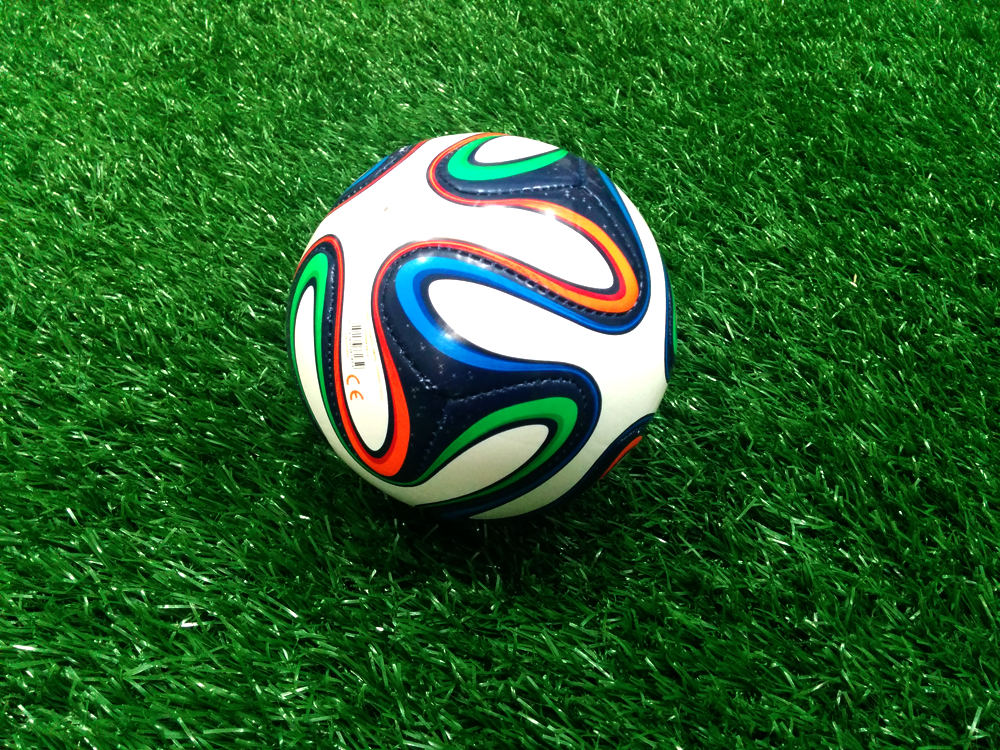
\includegraphics[width=0.3\textwidth]{images/fifa_ball}
			\caption{Ball that often could not be detected.}
			\label{fig:fifa_ball}
		\end{figure}


	\section{Conclusion and Future Work} {
	\label{sec:conclusion}

		% \todo{Haar features performed better than HOGS or LBP. LBP features performed better than HOGS. Increasing the proportion of negative images decreased the hit rate.}

		This paper approached the problem of sphere detection using boosted classifiers.
		We hypothesised that including a larger proportion of disk-like images as negative samples in the training set would increase the precision of the resulting sphere detectors.
		The hypothesis was tested in a controlled experiment that compared the appropriateness of three different feature types to the problem: extended Haar features, LBPs, and HoGs.
		The results of the experiment supported the hypothesis, but further testing would be required to have a high confidence that the increase in precision identified can be attributed to the increase in the proportion of disk-like negative images in the training set.
		Additionally, our results suggested that Haar features are better suited to the problem of sphere detection than LBPs.

		In our future work, we plan to repeat the experiment described in this paper with a greater number and variety of training schemes. We also plan to experiment with image preprocessing techniques, to investigate the effect they have on the precision of our sphere detector. These preprocessing techniques should be applied to both the positive and negative samples prior to training and upon classification. We will consider histogram equalisation, gamma intensity correction and high and low pass filtering \citep{gross2003image} as preprocessing techniques in our future work.

	}

	%
	% The following two commands are all you need in the
	% initial runs of your .tex file to
	% produce the bibliography for the citations in your paper.
	\bibliographystyle{abbrv}
	\bibliography{bibliography}  % sigproc.bib is the name of the Bibliography in this case
	% You must have a proper ".bib" file
	%  and remember to run:
	% latex bibtex latex latex
	% to resolve all references
	%
	% ACM needs 'a single self-contained file'!
	%

\end{document}
